\section{Physical Model}
\label{sec:model}

\subsection{Coordinates, the target plane, and the observations}

We place the origin at the centre of the penalty mark, with $x$ horizontal
towards the centre of the goal, $y$ across the goal, and $z$ vertically upwards
(Fig.~\ref{fig:geometry}). The ball is struck at $t=0$ with its centre at
$\vect r_0=(0,0,0.11)$ m, one radius above the ground. The goal is the plane
$x=x_g=11.0$ m, whose opening is $-b\le y\le b$ with $b=3.66$ m and
$0\le z\le h$ with $h=2.44$ m, a rectangle of $7.32$ m by $2.44$ m
\citep{ifab2025}. A goal counts only if the whole ball is past the line and
inside the frame. For a sphere of radius $R=0.110$ m this requires the centre at
the crossing to satisfy
\begin{equation}
  |y|\le b-R=3.55\ \text{m},
  \qquad
  R\le z\le h-R=2.33\ \text{m},
  \label{eq:clearance}
\end{equation}
because the sphere meets the plane in a disc of radius $R$. All probabilities in
this paper use this whole-ball convention, which treats the goal as a plane of
zero thickness and ignores contact with, or deformation of, the frame.

The method receives two measured positions of the ball centre,
$\vect r_1=(1.50,0.45,0.44)$ m at $t_1=0.05$ s and
$\vect r_2=(2.96,0.86,0.74)$ m at $t_2=0.10$ s (Fig.~\ref{fig:geometry}), and
returns the point where the trajectory crosses $x=x_g$. At the fitted launch
speed the crossing occurs at $t=0.3988$ s, so the fixes sample the first quarter
of the flight and everything beyond $0.10$ s is extrapolation. The task is
therefore not interpolation between fixes but out-of-sample continuation of a
trajectory whose aerodynamic force is itself unmeasured.

\begin{figure}[htbp]
  \centering
  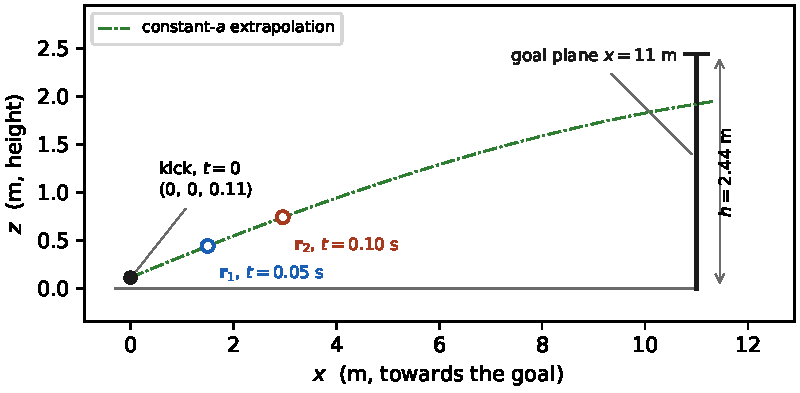
\includegraphics[width=0.61\textwidth]{f01-geometry.pdf}
  \caption{Geometry of the problem in the side view. The goal is the plane
  $x=11$ m with an opening $7.32$ m wide (not visible in this view) and
  $2.44$ m high. The filled circle is the kick point, the two open circles are
  the given observations $\vect r_1$ at $0.05$ s and $\vect r_2$ at $0.10$ s,
  and the dash-dot line is the constant-acceleration extrapolation retained as a
  control in \S\ref{sec:results}.}
  \label{fig:geometry}
\end{figure}

\subsection{Equations of motion and a transverse-force model}

We model the ball as a rigid sphere of mass $m=0.430$ kg and radius
$R=0.110$ m, with cross-section $A=\pi R^2=0.038013$ m$^2$, moving through air
of density $\rho=1.20$ kg m$^{-3}$ that may itself move with velocity $\vect w$.
Let $\vect u=\vect v-\vect w$ be the air velocity relative to the ball. The
equations of motion are
\begin{equation}
  \frac{\dd\vect v}{\dd t}
  =-\mathrm{FACTOR}\,C_D\,|\vect u|\,\vect u
  +|\vect u|\,(\vect\beta\times\vect u)
  -g\,\hat{\vect z},
  \qquad
  \frac{\dd\vect r}{\dd t}=\vect v,
  \label{eq:eom}
\end{equation}
where $g=9.81$ m\,s$^{-2}$, $\vect u=\vect v-\vect v_{\rm wind}$,
$\mathrm{FACTOR}=\rho A/(2m)=0.053042$ m$^{-1}$, and $\vect\beta$ is a
constant vector with units m$^{-1}$.

The first term is quadratic drag along $-\vect u$ \citep{mehta1985,nathan2008}.
Being parallel to the relative velocity, it changes the speed but not the
direction of motion in still air. The second term is the transverse force: its
magnitude is at most $|\vect\beta||\vect u|^2$ and its direction
$\vect\beta\times\vect u$ is perpendicular to $\vect u$, so it does no work in
still air. This is the form of the force on a spinning ball, for which
$\vect\beta$ points along the spin axis and its magnitude is proportional to the
spin at a given speed, and it also represents the side force on a non-spinning
ball whose wake is
asymmetric \citep{texier2016}, since for any direction perpendicular to $\vect u$
a suitable $\vect\beta$ produces it. The fit therefore determines the force
itself rather than the spin, and presupposes neither mechanism.

To expose the two independent directions of the force, we resolve $\vect\beta$
in a basis attached to the launch direction. Let $\vect u_0=\vect v_0-\vect w$,
$\vect e_0=\vect u_0/|\vect u_0|$,
$\vect e_1=(\hat{\vect z}\times\vect e_0)/|\hat{\vect z}\times\vect e_0|$,
which is horizontal and perpendicular to the flight plane, and
$\vect e_2=\vect e_0\times\vect e_1$, which lies in that plane. We write
\begin{equation}
  \vect\beta=\beta_1\vect e_1+\beta_2\vect e_2,
  \label{eq:beta}
\end{equation}
so that, by the cross product, $\beta_2$ drives the sideways force and $\beta_1$
the lift. The component of
$\vect\beta$ along $\vect e_0$ is omitted: at $t=0$ it produces no force, because
$\vect\beta\times\vect u_0=0$, and later it produces only a small force, because
the relative velocity turns by a few degrees during the flight.
Section~\ref{sec:method} shows that this component is also the one the data
cannot determine. The flight is then described by six parameters,
\begin{equation}
  \vect\theta=(\vect v_0,\,C_D,\,\beta_1,\,\beta_2),
  \label{eq:theta}
\end{equation}
the launch velocity, the drag coefficient, and the two transverse coefficients.
The nominal analysis takes still air, $\vect w=0$; uniform wind is reinstated as
a scenario in \S\ref{sec:method}, where it enters only through $\vect u$.

\subsection{Aerodynamic scales and the fitted coefficients}

The dimensionless groups are the Reynolds number $Re=U(2R)/\nu$ and the spin
parameter $S_p=\omega R/U$, with $U=|\vect u|$ the relative speed and
$\nu=1.5\times10^{-5}$ m$^2$ s$^{-1}$ the kinematic viscosity. At the penalty
speed $U\approx31$ m s$^{-1}$, $Re\approx4.4\times10^5$. The drag crisis of a
football occurs at $Re\approx(9$--$13)\times10^4$, that is $U\approx6$--$9$
m s$^{-1}$; above it $C_D$ is nearly flat at $0.17$--$0.22$
\citep{carre2005,goff2012}. The flight therefore lies well inside the flat
region, so a constant $C_D$ is a good approximation; the uncertainty is the
ball-to-ball scatter of its level, not the shape of $C_D(Re)$. That level is also
difficult to recover from a short trajectory: whole-trajectory estimates of
$C_D$ and $C_L$ can disagree with estimates from the local curvature and torsion
of the track \citep{jsme2014}, and trajectory-based drag estimates are sensitive
to the assumed force model \citep{florio2019}. We therefore fit $C_D$ with a
broad prior rather than fixing it from wind-tunnel data.

The transverse force is constrained by the same two fixes. Measurements give
lift coefficients $C_L=0.21$--$0.29$ at $S_p=0.18$--$0.34$ \citep{asai2020},
consistent with the linear law $C_L=C_{L0}S_p$ and $C_{L0}$ of order unity. In
the present parameterisation the equivalent lift coefficient is
$C_L=|\vect\beta|/\mathrm{FACTOR}$, which writes the transverse acceleration as
$C_L\rho A|\vect u|^2/(2m)$. The fitted value, $C_L=0.159$
(\S\ref{sec:method}), lies just below the measured range. Under the measured
linear law it is the force on a ball spinning at several revolutions per second
and corresponds to a transverse acceleration of the same order as gravity, the
scale on which a spinning or seam-oriented ball curves; it moves the crossing by
a distance large compared with the precision of the fixes. Table~\ref{tab:params} collects
the constants and Fig.~\ref{fig:aero} places the flight relative to the drag
crisis and the lift measurements.

\begin{table}[t]
  \centering
  \caption{Constants of the flight model. The last column gives the source of
  each value or the rule that fixes it. The position precision is a property of
  the printed coordinates, not a calibration of a tracking system.}
  \label{tab:params}
  \begin{tabular}{@{}llll@{}}
    \toprule
    Quantity & Symbol & Value used & Source or rule \\
    \midrule
    Air density (20\,\si{\degreeCelsius}, sea level) & $\rho$ & $1.20$ kg/m$^3$ & $\pm4\%$ \\
    Kinematic viscosity & $\nu$ & $1.5\times10^{-5}$ m$^2$/s & air at 20\,\si{\degreeCelsius} \\
    Ball radius & $R$ & $0.110$ m & circumference 68--70 cm \citep{ifab2025} \\
    Ball mass & $m$ & $0.430$ kg & 410--450 g \citep{ifab2025} \\
    Cross-section & $A$ & $3.8013\times10^{-2}$ m$^2$ & $\pi R^2$ \\
    Gravity & $g$ & $9.81$ m/s$^2$ & standard value \\
    Drag factor & $\mathrm{FACTOR}$ & $5.3042\times10^{-2}$ m$^{-1}$ & $\rho A/(2m)$ \\
    Position precision & $\sigma_{\rm pos}$ & $5$ mm & half the last printed digit \\
    \bottomrule
  \end{tabular}
\end{table}

\begin{figure}[htbp]
  \centering
  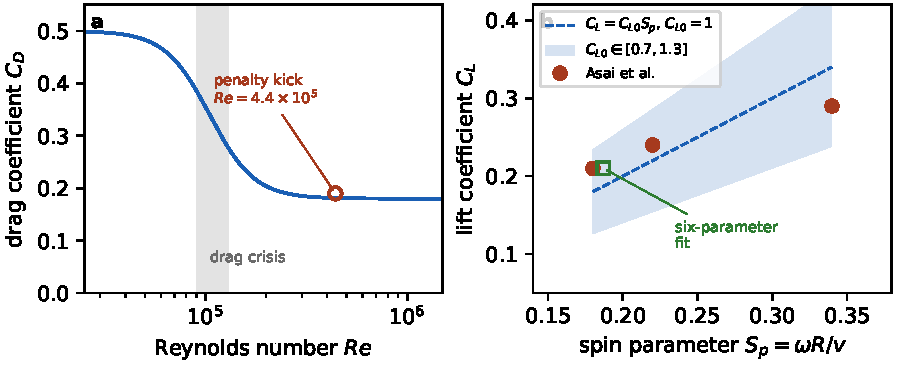
\includegraphics[width=0.68\textwidth]{f14-aero.pdf}
  \caption{Aerodynamic inputs. (a) The drag crisis of a football, shown as a
  guide to the eye through the values of \citep{carre2005,goff2012}: $C_D$ falls
  through $Re\approx(9$--$13)\times10^{4}$ and is flat above it. The open circle
  is the operating point of a penalty kick at $31$ m/s. (b) Lift coefficient
  against spin parameter: the model's $C_L=C_{L0}S_p$ with $C_{L0}=1$ and its
  $0.7$--$1.3$ band (dashed and shaded), the measurements of \citep{asai2020}
  (filled circles), and the spin parameter of the earlier spinning-ball fit
  retained as a control (\S\ref{sec:results}).}
  \label{fig:aero}
\end{figure}

\subsection{Drag alone cannot bend the shot}

The model has a structural property that organises the analysis. With drag and
gravity only, and still air, the horizontal equation is
$\dot{\vect v}_\perp=-k|\vect v|\vect v_\perp$ with $k=\mathrm{FACTOR}\,C_D>0$.
Both components of $\vect v_\perp$ are multiplied by the same positive scalar,
so their ratio is conserved:
\begin{equation}
  \frac{\dd}{\dd t}\left(\frac{v_y}{v_x}\right)=0
  \quad\Longrightarrow\quad
  \frac{y(t)}{x(t)}=\frac{v_{0y}}{v_{0x}}
  \quad\Longrightarrow\quad
  y_{\rm entry}=x_g\,\frac{v_{0y}}{v_{0x}},
  \label{eq:nobend}
\end{equation}
independently of the magnitude of the drag and, indeed, of any drag law that
depends only on speed. Drag changes the flight time and the height at the plane,
but it cannot move the crossing sideways relative to the initial aim; only a
force with a component perpendicular to $\vect v$ can. This is why the
transverse coefficients, not $C_D$, control the lateral prediction.

The data show the same structure. A drag-and-gravity model fitted to the six
numbers returns $y=3.2172$ m at the plane, whereas the exact
constant-acceleration fit of the same numbers returns $y=2.4948$ m. Both
reproduce the fixes to within their precision, which is precisely the
difficulty: two fixes alone can barely separate the two descriptions, and no
choice of $C_D$ can close the gap, because the drag-only crossing is tied to
$x_gv_{0y}/v_{0x}$ by Eq.~\eqref{eq:nobend}. A uniform wind breaks the identity,
since drag is then along $\vect u$ rather than $\vect v$, but over the $0.1$ s
baseline it is nearly degenerate with the launch velocity and the refit absorbs
most of it (\S\ref{sec:method}). The lateral answer is therefore an inference,
not a measurement.

\subsection{Numerical integration and the target-plane crossing}

The state $\vect s=(\vect r,\vect v)$ is advanced with the classical
fourth-order Runge--Kutta scheme
\begin{equation}
  \vect s_{n+1}=\vect s_n+\frac{\Delta t}{6}\left(\vect f_1+2\vect f_2+2\vect f_3+\vect f_4\right)
  +\order{\Delta t^5},
  \label{eq:rk4}
\end{equation}
at the fixed step $\Delta t=0.005$ s. The crossing of $x=x_g$ is located by
cubic Hermite interpolation of $x(t)-x_g$ across the bracketing step, using the
position and velocity supplied at both ends; since the interpolant matches both
values and both derivatives, its error is $\order{\Delta t^4}$, the same order
as the integration. Halving $\Delta t$ changes the entry ordinates by less than
$1$ mm, far below the $5$ mm precision of the fixes and the spread of the
prediction. The same integrator and crossing rule are used in the fit and in the
prediction, so no interpolation of the model enters between the two stages.
